\documentclass[12pt]{article}

\usepackage{fullpage,natbib,amsmath,setspace,graphicx}
\usepackage{wrapfig}
\usepackage{lscape}
\usepackage{rotating}
\usepackage{epstopdf}

\title{Evaluating the Impact of Context Specific Factors on ELO Ratings' Predictive Validity}
\author{Mitchell Goist and Ryan McMahon}
\date{3 May 2016}

\begin{document}
\maketitle

\doublespacing
\section{Motivation}

Over the past decade, predictive analytics have risen to importance within sports analysis. Sports represents an ideal application for these methods, as predicting outcomes is far more important than generating causal inferences about the particular effect each feature has on the outcome. Another trend in sports analysis is its popular consumption; more and more people are becoming interested in quantitative ways to understand their favorite sports. In order to ``democratize'' access, an increased emphasis has been placed on single variable indices of quality, which are much easier to understand than multidimensional representations.

Therefore, sports analysts face a trade-off between interpretability, on the one hand, and predictive validity, on the other. This paper attempts to measure that trade-off by evaluating the predictive validity of one of the more popular single-variable metrics for team quality: ELO ratings. ELO is used in a wide variety of contexts. It originated with Chess rankings, but has expanded to american football, soccer, and cricket. 

The ELO rating has many properties which make it ideally suited for a single-variable metric. First, it is updated after every game, and is zero-sum, implying that for every points the winning team gains, the losing team loses a corresponding amount. Second, the parameters can be adjusted to account for both margin of victory and sensitivity to past results.

It is defined as follows. Player A has a rating of $R_{a}$, and Player B has a rating of $R_{b}$. The ELO of Player A is updated as $E_{a} = \dfrac{1}{1+10^{R_{b}-R_{a}/400}}$, and correspondingly for player B. This is updated dynamically as $R_{a(n)} = R_{a(n-1)} + K(1-E_{a(n-1)}$. It can be seen here, that as the parameter $K$, the ratings become more sensitive to recent results. A popular implementation, by the blog FiveThirtyEight, adjusts this original formula to accomodate for margin of victory, rather than a simple binary distinction between wins and losses. This is calculated as $\dfrac{(MOV + 3)^{0.8}}{7.5 + 0.006 x ELO_{diff}}$, which produces a fraction that scales the $K$ parameter previously discussed.

The goal of this paper is to evaluate how much predictive validity is lost when games are predicted solely from their ELO ratings. As such, we will compare one model, where games are mechanically predicted by ELO, and another model, in which we incorporate a wide variety of context--specific features that are likely to impact the game outcomes. The paper proceeds as follows. First, we discuss our data and features; second, we compare a variety of classifiers for performance; and finally, we discuss our results. We conclude that the context features we add do not represent a dramatic improvement over the adjusted ELO rating.

\section{Data and Feature Selection}

In order to measure contextual effects on NBA outcomes, we needed to acquire statistics and game information for each game played over the most recent (2015-2016) season. The raw data was scraped from the NBA website. Our outcome measure, what we attempt to classify, is a binary indicator of win or loss. We selected a wide variety of features from the available data. The first concerns the location, attendance, and opponent. Home games are considered to create a considerable advantage, large attendance indicates raucous crowds that might amplify this advantage, and opponent dummies are necessary to determine whether favorable match-ups increase a team's chance of winning. The second set of features concerns what are typically called counting stats. These quantify the number of rebounds, points, assists, and other metrics that are collected for each team. Their inclusion is straightforward: teams with more points, rebounds,se or a higher shooting percentage, for example, are more likely to win the game. Third, we collected advanced or composite statistics generated by the NBA. These include proprietary measures of offensive and defensive efficiency, which are difficult to calculate through the use of counting statistics alone. Finally, we collected information on lineups, to test time effects of continuity between different configurations of players. All together, we had 72 features.

Before moving to classifiers and prediction results, there is an issue with predicting outcomes. Each observation in our data set is a team--game, where a loss is recorded as 0 and a win is recorded as 1. Of course, that team plays another team, which is also in our dataset under the same game. These are clearly not independent; in fact, there is a deterministic relationship within games, where one team's loss necessitates another team's win, and vice versa. One way to address this is through random sampling the games, and then bootstrapping, looping through all possible combinations until each unique team--game observation has been predicted at least once. However, this would be computationally intensive. In order to determine whether this sampling strategy would be worthwhile, we tested it with the ELO ratings, which generate mechanical predictions, and are therefore easy to compute. We found no substantive difference between taking one random sample of all games within pairs, and the bootstrapping method outlined previously. Therefore, we simply took a random sample within pairs, providing us with 1230 observations.


\section{Classifier Comparison}

We were \emph{a priori} unsure of which classifier would provide us with the best performance. Instead, we tried using multiple approaches: logistic regression with L1 penalties; logistic regression with L2 penalties; Bernoulli Naive Bayes; AdaBoost; SVM; and Random Forest Regression. We then compared the methods based on their predictive accuracy. Before discussing our results, we will briefly describe the mechanics behind each classifier, and their relative advantages and disadvantages.

\subsection{Logistic Regression with L1 Penalties}

The first, and most obvious, classifier to use for a problem with a binary outcome is logistic regression. Because we have so many features, we use L1 penalties to avoid overfitting \citep{tibshirani}. L1 penalties sum up the absolute values for the weights of each feature. This produces sparse feature sets. This might be useful in our setting, because many of the counting stats could be redundant. All regularization procedures are designed to find weight coefficients so that the cost function is minimized. In practice, this means that many of the coefficients when using an L1 penalty will be driven close to zero. This can be formally written as: $min(Y - X_{w})^{T}(Y-X_{w}) + \lambda\sum_{i=1}^{n}|w_{i}|$. While L1 penalties have some desirable properties, this might not be entirely appropriate, due to a lack of sparsity in our data.

\subsection{Logistic Regression with L2 Penalties}

In addition to L1 penalties, we also employ logistic regression with L2 penalties. This functions differently from the L1 penalties, as it does not assume sparsity, and instead keeps many of the coefficients above zero. The set-up is very similar to L1 regression, in that you still select weight coefficients to minimize the cost function \citep{hoerl}. The difference is that L1 penalties uses the sum of absolute values, whereas L2 penalties simply square the weights, and then sum them (using a similar equation to the one previous described for L1 penalties). Because L1 adjusts for sparsity, whereas L2 encourages many features, both have the potential to be appropriate, depending on the nature of the relationship.

\subsection{Bernoulli Naive Bayes}

Another simple to employ classifier is Naive Bayes, adapted, in this case, to the Bernoulli setting for our binary outcome variable. Naive Bayes works by updating the prior distribution with data from each feature, producing a posterior that can be checked for predictive accuracy. In the Bernoulli case, this can be formally written as $\hat{y} = argmax\thinspace p(C_{k})\prod_{i=1}^{n}(p_{x_{i}}|c)$ \citep{mccallum}. We employ Naive Bayes for its simplicity and computaiton ease, which make it an appropriate baseline model. However, we do not suspect it will perform well, due to the independenc assumption between features.

\subsection{SVM}

Support Vector Machines (SVMs) are another commonly used classifier, based on the original perceptron model. SVMs work by first finding the support vectors, which are the training samples closes to the hyperplane, and the maximizing the distance between this hyperplane and the support vectors. We employ a least squares version of the SVM, using the L1 norm previously described \citep{suykens}.
 
\subsection{AdaBoost}

Our next classifier we test, is not technically a single classifier, but rather an ensemble method that leverages many weak classifiers. These classifiers learn from the training sample and lead to better predictions in the ensemble \citep{breiman}. Specifically, we use Adaboost, which employs decision tree stumps as weak learners, and weights them by minimizing the cost function over multiple rounds \citep{ratsch}. 

\subsection{Random Forest Regression}

Our final classifier are random forests. While not often considered as such, these can be thought of as another ensemble learning technique, where the predictions from multiple decision trees are combined and weighted. This is done through bagging, which is a typical ensemble learning method. Random forests are a very flexible and robust method, and with our modestly sized featured set, should not be overly burdensome computationally.

\section{Discussion}
Figures 1 and 2 display our results. We made two comparisons, as described in the Motivation section. The first is to compare our classifiers against a mechanical prediction made by the ELO ratings, adjusted, according to the methodology used by 538 and described earlier, for home court advantage. Figure 2 compares the non-home court adjusted ELO ratings to our classifiers. Because L2 logistic regression was outperformed consistently by L1 penalties, we decided to only include one of the logistic regression classifiers in our figures.

\begin{sidewaysfigure}[p!]
\caption{538 ELO Classifier Comparison}
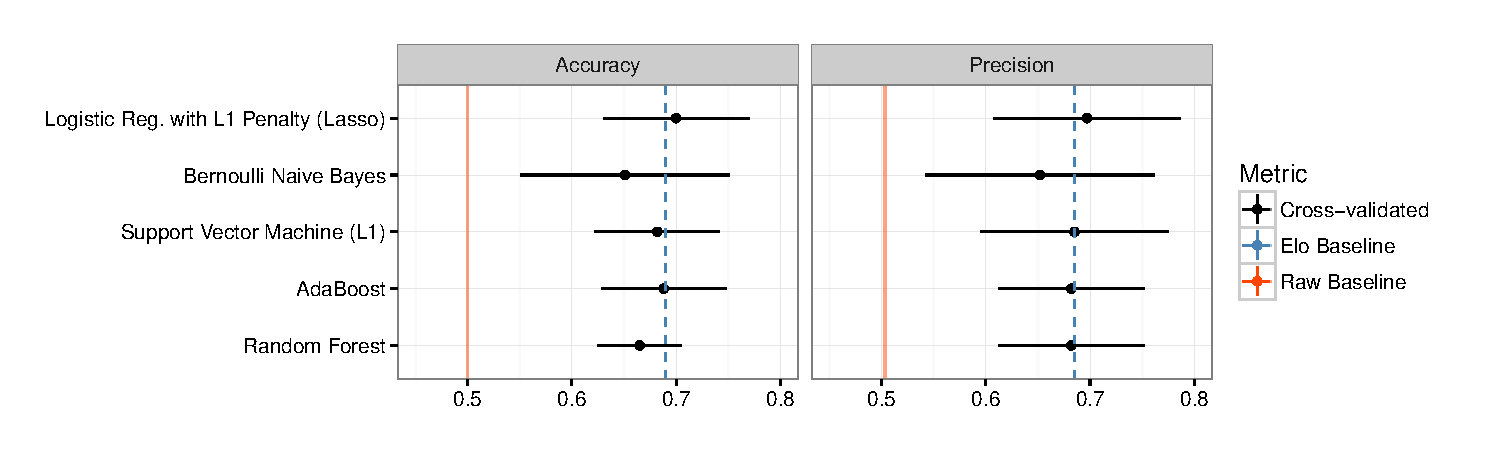
\includegraphics[]{01a-538-classifier-comparison.pdf}
\end{sidewaysfigure}

\begin{sidewaysfigure}[p!]
\caption{Non-home courd adjusted ELO classifier Comparison}
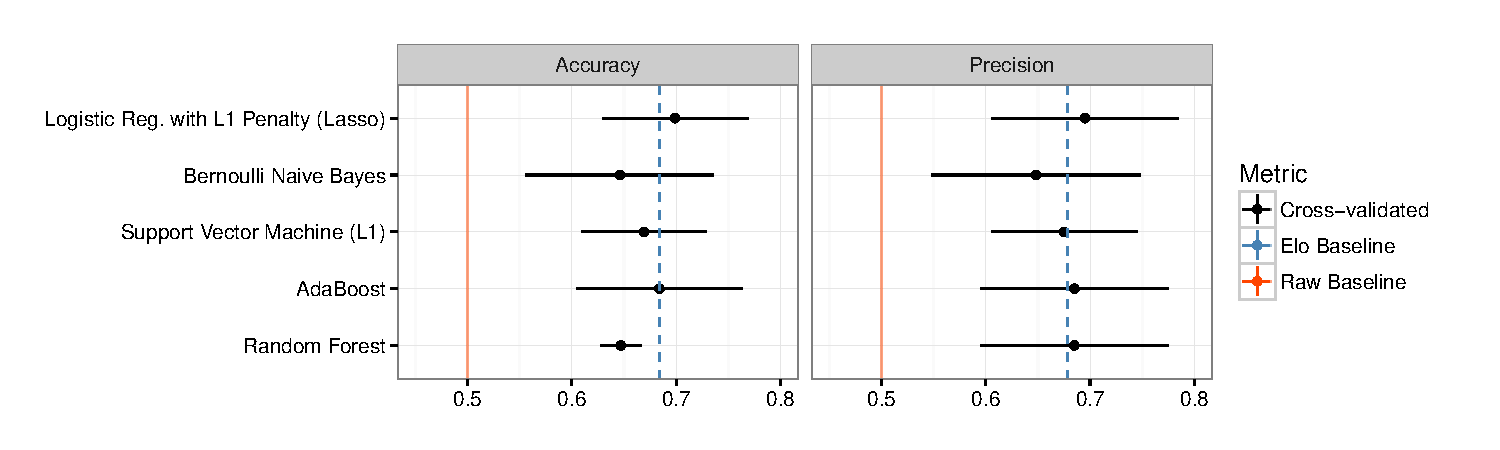
\includegraphics[]{01b-no-hc-classifier-comparison.pdf}
\end{sidewaysfigure}

There are two primary conclusions. First LASSO, or logistic regression with L1 penalties, outperformed all of the other classifiers. This leads us to believe that we do, indeed have a sparse feature set, and any of the potential gains from the ensemble methods or SVM were not useful in this context. Naive Bayes performed, by far, the worse. This was to be expected, as our features clearly violate the independence assumption necessary for that classifier to work properly.

The second main conclusion is that, surprisingly, the ELO system does a very good job at predicting games, particularly using the 538 adjustment for home court advantage. The modest gains received from our best classifier, logistic regression with L1 penalties, are likely outweighed by ELO's parsimony and ease of explanation. This lack of improvement also suggests that there is a limit to how predictable NBA games are. Predicting sporting contests has long been the primary goal of sports analysis, but there exists a large stochastic or chaotic component in these games that is difficult for any feature set to fully incorporate and judge. We therefore recommend that ELO be used with the 538 homecourt adjustment, and that foregoing other contextual features does not lead to a significant decline in predictive validity.

\section*{Appendix: Code}

\begin{verbatim}
import numpy as np
import pandas as pd
import os


#######################
## Pre-processing:
#######################
from sklearn.preprocessing import MinMaxScaler
from sklearn.preprocessing import OneHotEncoder

# drop out NAs
elo538.dropna(axis=0, how='any', inplace=True)

# separate out our DV:
y = np.array(elo538.win_dum)

# remove the DV, game IDs, and ref IDs from the data frame:
elo538.drop(['win_dum', 'X_iscopy', 'game_id', 'date_game', 'ref_id1', 'ref_id2', 'ref_id3'], 
axis=1, inplace=True)


# dummy out string variables:
elo538 = pd.get_dummies(elo538)
X = elo538


# normalize numeric data:
mms = MinMaxScaler()
X_norm = mms.fit_transform(X)
X_norm = pd.DataFrame(X_norm)
X_norm.columns = X.columns.values


#######################
## Logistic Regression:
#######################

from sklearn import cross_validation
from sklearn.linear_model import LogisticRegression

print 'Estimating regularization parameter via cross-validation...'
## choosing regularization parameter with cross-validation
alphas = [0.0001, 0.0005, 0.001, 0.005, 0.01, 0.05, 0.1, 0.125, 0.15, 0.2]
val = alphas[0]
max_score = 0

for a in alphas:
clf_logit1 = LogisticRegression(penalty="l1", C=a)
clf_logit1.fit(X_norm, y)
scores = cross_validation.cross_val_score(clf_logit1, X_norm, y, cv=10)
print str(a) + ':' + str(scores.mean())
if scores.mean() > max_score:
val = a
max_score = scores.mean()


print 'Fitting classifier with alpha=' + str(val)
clf_logit1 = LogisticRegression(penalty="l1", C=val)

scores = cross_validation.cross_val_score(clf_logit1, X_norm, y, cv=10)
precision = cross_validation.cross_val_score(clf_logit1, X_norm, y, cv=10, scoring='precision')


from collections import Counter
freqs = Counter(y)

print("Accuracy: %0.3f (+/- %0.2f)" % (scores.mean(), scores.std() * 2))
print("Baseline accuracy (all 0's): %0.2f" % (float(freqs[0]) / len(y)))
print("Baseline accuracy (all 1's): %0.2f" % (float(freqs[1]) / len(y)))
print("Precision: %0.3f (+/- %0.2f)" % (precision.mean(), precision.std() * 2))


clf_logit1.fit(X_norm, y)

def show_most_informative_features(words, clf, n=20):
c_f = sorted(zip(clf.coef_[0], words))
top = zip(c_f[:n], c_f[:-(n+1):-1])
print "\t%.4s\t%-20s\t\t%.4s\t%-20s" % ("","NEGATIVE","","POSITIVE")
for (c1,f1),(c2,f2) in top:
print "\t%.4f\t%-25s\t\t%.4f\t%-25s" % (c1,f1,c2,f2)

show_most_informative_features(X_norm.columns.values, clf_logit1, n=25)

#######################
# Naive Bayes
######################

from sklearn.naive_bayes import BernoulliNB

print 'Estimating regularization parameter via cross-validation...'
## choosing regularization parameter with cross-validation
alphas = [0.001, 0.005, 0.01, 0.05, 0.1, 0.2]
val = alphas[0]
max_score = 0

for a in alphas:
classifier = BernoulliNB(alpha=a)
classifier.fit(X_norm, y)
scores = cross_validation.cross_val_score(classifier, X_norm, y, cv=5)
print str(a) + ':' + str(scores.mean())
if scores.mean() > max_score:
val = a
max_score = scores.mean()

## running classifier
print 'Fitting classifier with alpha=' + str(val)
classifier = BernoulliNB(alpha=val)

print "\nBernoulli Naive Bayes\n"

scores = cross_validation.cross_val_score(classifier, X_norm, y, cv=10)
precision = cross_validation.cross_val_score(classifier, X_norm, y, cv=10, scoring='precision')
#recall = cross_validation.cross_val_score(classifier, X, y, cv=10, scoring='recall', n_jobs=10)

from collections import Counter
freqs = Counter(y)

print("Accuracy: %0.3f (+/- %0.2f)" % (scores.mean(), scores.std() * 2))
print("Baseline accuracy (all 0's): %0.2f" % (float(freqs[0]) / len(y)))
print("Baseline accuracy (all 1's): %0.2f" % (float(freqs[1]) / len(y)))
print("Precision: %0.3f (+/- %0.2f)" % (precision.mean(), precision.std() * 2))
#print("Recall: %0.3f (+/- %0.2f)" % (recall.mean(), recall.std() * 2))

classifier.fit(X_norm, y)

def show_most_informative_features(words, clf, n=20):
c_f = sorted(zip(clf.coef_[0], words))
top = zip(c_f[:n], c_f[:-(n+1):-1])
print "\t%.4s\t%-20s\t\t%.4s\t%-20s" % ("","NEGATIVE","","POSITIVE")
for (c1,f1),(c2,f2) in top:
print "\t%.4f\t%-25s\t\t%.4f\t%-25s" % (c1,f1,c2,f2)

show_most_informative_features(X_norm.columns.values, classifier, n=25)




#######################
# SVM
######################

print "\nSVM\n"

from sklearn.svm import LinearSVC

print 'Estimating regularization parameter via cross-validation...'
## choosing regularization parameter with cross-validation
alphas = [0.01, 0.05, 0.10, 0.50, 0.75, 1, 1.50]
val = alphas[0]
max_score = 0

# l2 penalty has better cross-validated performance
for a in alphas:
classifier = LinearSVC(C=a, penalty='l2')
classifier.fit(X_norm, y)
scores = cross_validation.cross_val_score(classifier, X_norm, y, cv=10)
print str(a) + ':' + str(scores.mean())
if scores.mean() > max_score:
val = a
max_score = scores.mean()

## running classifier
print 'Fitting classifier with alpha=' + str(val)
classifier = LinearSVC(C=val)


scores = cross_validation.cross_val_score(classifier, X_norm, y, cv=10)
precision = cross_validation.cross_val_score(classifier, X_norm, y, cv=10, scoring='precision')


from collections import Counter
freqs = Counter(y)

print("Accuracy: %0.3f (+/- %0.2f)" % (scores.mean(), scores.std() * 2))
print("Baseline accuracy (all 0's): %0.2f" % (float(freqs[0]) / len(y)))
print("Baseline accuracy (all 1's): %0.2f" % (float(freqs[1]) / len(y)))
print("Precision: %0.3f (+/- %0.2f)" % (precision.mean(), precision.std() * 2))



classifier.fit(X_norm, y)



#######################
# Adaboost
######################

print "\nAdaboost\n"

### Adaboost
from sklearn.ensemble import AdaBoostClassifier

n_ests = [5, 10, 25, 50, 100, 250]
rates = [0.01, 0.05, 0.10, 0.25, 0.50]
val_est = n_ests[0]
val_rate = rates[0]
max_score = 0

for n in n_ests:
for r in rates:
classifier = AdaBoostClassifier(n_estimators=n, learning_rate=r, random_state=0)
classifier.fit(X_norm, y)
scores = cross_validation.cross_val_score(classifier, X_norm, y, cv=10)
print str(n) + ' estimators & ' + str(r) + ' rate= ' + str(scores.mean())
if scores.mean() > max_score:
val_est = n
val_rate = r
max_score = scores.mean()

## running classifier
print 'Fitting classifier with n_estimators=' + str(val_est) + ' & ' + ' learning rate=' + str(val_rate) 

classifier = AdaBoostClassifier(n_estimators=val_est, learning_rate=val_rate, 
random_state=0)

scores = cross_validation.cross_val_score(classifier, X_norm, y, cv=10)
precision = cross_validation.cross_val_score(classifier, X_norm, y, cv=10, scoring='precision')


from collections import Counter
freqs = Counter(y)

print("Accuracy: %0.3f (+/- %0.2f)" % (scores.mean(), scores.std() * 2))
print("Baseline accuracy (all 0's): %0.2f" % (float(freqs[0]) / len(y)))
print("Baseline accuracy (all 1's): %0.2f" % (float(freqs[1]) / len(y)))
print("Precision: %0.3f (+/- %0.2f)" % (precision.mean(), precision.std() * 2))




#######################
# Random Forest
#######################

print "\nRandom Forest\n"

n_ests = [250, 500, 1000, 2000]
n_depth = [2, 3, 4, 5, 8, 10]

val_est = n_ests[0]
val_dep = n_depth[0]
max_score = 0

from sklearn.ensemble import RandomForestClassifier
for n in n_ests:
for d in n_depth:
classifier = RandomForestClassifier(n_estimators=n, random_state=0, 
max_depth=d)
classifier.fit(X_norm, y)
scores = cross_validation.cross_val_score(classifier, X_norm, y, cv=5)
print str(n) + ' estimators w/ ' + str(d) + ' depth= ' + str(scores.mean())
if scores.mean() > max_score:
val_est = n
val_dep = d
max_score = scores.mean()


## running classifier
print 'Fitting classifier with n_estimators=' + str(val_est) + ' and a max depth of ' + str(val_dep)

classifier = RandomForestClassifier(n_estimators=val_est, random_state=0, 
max_depth=val_dep)

from collections import Counter
freqs = Counter(y)

print("Accuracy: %0.3f (+/- %0.2f)" % (scores.mean(), scores.std() * 2))
print("Baseline accuracy (all 0's): %0.2f" % (float(freqs[0]) / len(y)))
print("Baseline accuracy (all 1's): %0.2f" % (float(freqs[1]) / len(y)))
print("Precision: %0.3f (+/- %0.2f)" % (precision.mean(), precision.std() * 2))




classifier.fit(X_norm, y)

\end{verbatim}

\bibliographystyle{plain}
\bibliography{ist597k}


\end{document}
